\documentclass[11pt,a4paper,oneside]{report}

% Jerry project software documentation.
% Compile from the repository root with pdfLaTeX twice to populate the TOC:
% pdflatex -interaction=nonstopmode docs/jerry-software-documentation.tex
% pdflatex -interaction=nonstopmode docs/jerry-software-documentation.tex

\usepackage[utf8]{inputenc}
\usepackage[T1]{fontenc}
\usepackage{lmodern}
\usepackage[a4paper,margin=25mm,headheight=15pt]{geometry}
\usepackage{microtype}
\usepackage{graphicx}
\usepackage{xcolor}
\usepackage{tikz}
\usetikzlibrary{arrows.meta,positioning,calc}
\usepackage{booktabs}
\usepackage{longtable}
\usepackage{tabularx}
\usepackage{array}
\usepackage{enumitem}
\usepackage{listings}
\usepackage{fancyhdr}
\usepackage{caption}
\usepackage{float}
\usepackage{hyperref}
\usepackage{bookmark}

\definecolor{JerryNavy}{HTML}{17324D}
\definecolor{JerryBlue}{HTML}{3474BD}
\definecolor{JerryTeal}{HTML}{16856B}
\definecolor{JerryLight}{HTML}{EEF4FA}
\definecolor{JerryGray}{HTML}{596D82}
\definecolor{JerryCode}{HTML}{F3F6F9}

\hypersetup{
  colorlinks=true,
  linkcolor=JerryBlue,
  urlcolor=JerryBlue,
  citecolor=JerryTeal,
  pdftitle={Jerry - Software Documentation},
  pdfsubject={Architecture, operation, API, security, and testing reference for Jerry},
  pdfauthor={Jerry Project}
}

\graphicspath{{docs/img/}{img/}}
\setlength{\parindent}{0pt}
\setlength{\parskip}{5pt plus 1pt}
\setlist[itemize]{leftmargin=1.5em,itemsep=2pt,topsep=3pt}
\setlist[enumerate]{leftmargin=1.7em,itemsep=3pt,topsep=4pt}
\setlength{\tabcolsep}{5pt}
\renewcommand{\arraystretch}{1.15}

\pagestyle{fancy}
\fancyhf{}
\fancyhead[L]{\small\textcolor{JerryGray}{Jerry | Software Documentation}}
\fancyhead[R]{\small\textcolor{JerryGray}{Local demo reference}}
\fancyfoot[L]{\small\textcolor{JerryGray}{Jerry project}}
\fancyfoot[R]{\small\textcolor{JerryGray}{\thepage}}
\renewcommand{\headrulewidth}{0.4pt}
\renewcommand{\footrulewidth}{0pt}

\lstdefinestyle{jerrycode}{
  basicstyle=\ttfamily\small,
  backgroundcolor=\color{JerryCode},
  frame=single,
  rulecolor=\color{JerryLight},
  breaklines=true,
  columns=fullflexible,
  keepspaces=true,
  showstringspaces=false,
  xleftmargin=7pt,
  xrightmargin=7pt,
  aboveskip=8pt,
  belowskip=8pt
}
\lstset{style=jerrycode}

\newcommand{\code}[1]{\texttt{\detokenize{#1}}}
\newcommand{\featurestatus}[1]{\textcolor{JerryTeal}{\textbf{#1}}}
\newcolumntype{Y}{>{\raggedright\arraybackslash}X}
\newcolumntype{L}[1]{>{\raggedright\arraybackslash}p{#1}}

\title{\textcolor{JerryNavy}{\Huge Jerry}\[5pt]
  \Large Enterprise Knowledge Assistant\\[8pt]
  \large Software Architecture and User Documentation}
\author{Jerry Project}
\date{Project reference | November 2026}

\begin{document}

% Cover
\begin{titlepage}
  \centering
  \vspace*{20mm}
  {\color{JerryBlue}\rule{0.92\textwidth}{2pt}}\\[17mm]
  {\color{JerryNavy}\Huge\bfseries Jerry\par}
  \vspace{5mm}
  {\LARGE Enterprise Knowledge Assistant\par}
  \vspace{4mm}
  {\large Software Architecture and User Documentation\par}
  \vspace{15mm}
  {\large A technical reference for the local demonstration application\par}
  \vfill
  \begin{tabular}{@{}ll@{}}
    Document revision: & 1.1 \\
    Reference date: & November 2026 \\
    Application branch model: & feature development through testing and production \\
    Primary interfaces: & Streamlit user interface and FastAPI service
  \end{tabular}
  \vspace{12mm}
  {\color{JerryBlue}\rule{0.92\textwidth}{1pt}}\\[4mm]
  {\small This document describes the repository implementation and its demo limitations.}
\end{titlepage}

\pagenumbering{roman}
\chapter*{Document control}
\addcontentsline{toc}{chapter}{Document control}
\begin{tabularx}{\textwidth}{@{}L{34mm}Y@{}}
\toprule
\textbf{Item} & \textbf{Description} \\
\midrule
Purpose & Explain the architecture, installation, operation, interfaces, safeguards, and test evidence for Jerry. \\
Audience & Project maintainers, evaluators, developers, and users running the local demo. \\
System scope & Python packages at the repository root, the Streamlit UI, FastAPI API, local sample documents, and optional hosted adapters. \\
Status & Assignment/demo reference. This is not a production security or service-level commitment. \\
Source set & The README, Markdown design notes in \code{docs/}, configuration template, API schemas, and the bundled example corpus. \\
\bottomrule
\end{tabularx}

\chapter*{How to use this document}
\addcontentsline{toc}{chapter}{How to use this document}
The table of contents is linked. Select a chapter title in the PDF to navigate to that section. The document is organized from system context and setup through runtime behavior, interfaces, security, testing, and operational limitations. Code font marks file names, commands, environment variables, endpoints, and schema fields.

\tableofcontents
\clearpage
\pagenumbering{arabic}

\chapter{Executive overview}

Jerry is a demonstration enterprise knowledge assistant for questions about internal policies, incident records, runbooks, and architecture notes. The user interface is built with Streamlit. A FastAPI service authenticates demo requests, applies rate limits and request validation, and calls a LangGraph workflow. The assistant retrieves passages from a small indexed corpus, applies evidence and citation checks, and returns an answer with source identifiers and workflow activity.

The default configuration is local-first. Sample Markdown documents are chunked and indexed into a local JSON Lines file. The default local feature-hash embedding is a repeatable demo representation; it is not a semantic embedding. With the local embedding provider, search uses BM25 keyword retrieval. OpenAI embeddings, Pinecone, an OpenAI chat model, and LangSmith tracing are optional integrations.

\section{Goals}
The implementation demonstrates:
\begin{itemize}
  \item document loading, metadata validation, chunking, indexing, and source-aware retrieval;
  \item explicit assistant routing, evidence checking, bounded retry, grounded responses, and citation validation;
  \item bounded incident analysis, session memory, server-side demo-role checks, and local tool wrappers;
  \item input validation, prompt-injection screening, per-user rate limiting, safe error responses, trace IDs, and streamed activity.
\end{itemize}

\section{Important scope limits}
Jerry is not a production banking assistant. Demo accounts are token-mapped sample identities, memory and rate limits are process-local, the local corpus is fictional and small, the local RLM analysis uses deterministic text patterns, and MCP-style data is served by local wrappers rather than a connected MCP server. Guardrails reduce risk but do not prevent all prompt injection or misuse. External services must be separately configured and evaluated.

\chapter{System architecture}

\section{Component model}
The Python package boundary is the repository root; the packages are not nested under an \code{app/} directory. The principal components and runtime paths are shown in Figure~\ref{fig:architecture}.

\begin{figure}[H]
\centering
\resizebox{\textwidth}{!}{%
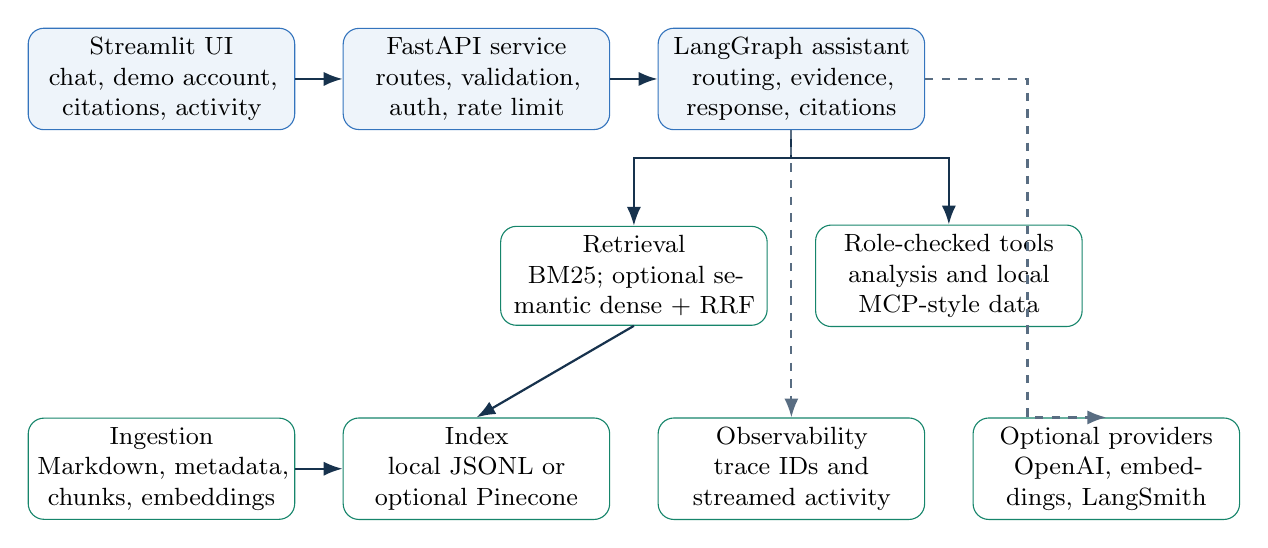
\begin{tikzpicture}[
  component/.style={draw=JerryBlue,fill=JerryLight,rounded corners=2mm,
    text width=3.15cm,minimum height=1.25cm,align=center,font=\small},
  support/.style={draw=JerryTeal,fill=white,rounded corners=2mm,
    text width=3.15cm,minimum height=1.25cm,align=center,font=\small},
  runtime/.style={-{Latex[length=2.4mm]},thick,draw=JerryNavy},
  optional/.style={-{Latex[length=2.4mm]},thick,dashed,draw=JerryGray}
]
\node[component] (ui) at (-4,2.7) {Streamlit UI\\chat, demo account, citations, activity};
\node[component] (api) at (0,2.7) {FastAPI service\\routes, validation, auth, rate limit};
\node[component] (graph) at (4,2.7) {LangGraph assistant\\routing, evidence, response, citations};
\node[support] (retrieval) at (2,0.2) {Retrieval\\BM25; optional semantic dense + RRF};
\node[support] (tools) at (6,0.2) {Role-checked tools\\analysis and local MCP-style data};
\node[support] (ingest) at (-4,-2.25) {Ingestion\\Markdown, metadata, chunks, embeddings};
\node[support] (index) at (0,-2.25) {Index\\local JSONL or optional Pinecone};
\node[support] (observe) at (4,-2.25) {Observability\\trace IDs and streamed activity};
\node[support] (providers) at (8,-2.25) {Optional providers\\OpenAI, embeddings, LangSmith};
\draw[runtime] (ui.east) -- (api.west);
\draw[runtime] (api.east) -- (graph.west);
\draw[runtime] (graph.south) -- ++(0,-0.35) -| (retrieval.north);
\draw[runtime] (graph.south) -- ++(0,-0.35) -| (tools.north);
\draw[runtime] (retrieval.south) -- (index.north);
\draw[runtime] (ingest.east) -- (index.west);
\draw[optional] (graph.south) -- ++(0,-1.2) -| (observe.north);
\draw[optional] (graph.east) -- ++(1.3,0) |- (providers.north);
\end{tikzpicture}%
}
\caption{Jerry components and the primary request, retrieval, and data paths. Solid arrows show the main runtime flow; dashed arrows mark supporting or optional integrations.}
\label{fig:architecture}
\end{figure}

\section{Development container topology}
Docker Compose defines \code{api}, \code{ui}, and \code{ingest} services from the root \code{Dockerfile}. API and UI bind-mount project source at \code{/workspace}; Uvicorn uses \code{--reload}. Compose publishes the API on host port 8010 and Streamlit on 8501, configurable with \code{JERRY_API_PORT} and \code{JERRY_UI_PORT}. The UI calls the API at \code{http://api:8010}; the API health check gates UI startup. Ingestion uses local embeddings and indexing, writing \code{data/local_index.jsonl} to the bind mount. This development setup is not production-hardened.

\section{Package responsibilities}
\begin{longtable}{@{}L{30mm}L{42mm}L{75mm}@{}}
\toprule
\textbf{Package} & \textbf{Responsibility} & \textbf{Representative modules} \\
\midrule
\endfirsthead
\toprule
\textbf{Package} & \textbf{Responsibility} & \textbf{Representative modules} \\
\midrule
\endhead
\code{api/} & HTTP application, routes, dependencies, exception mapping & \code{api/main.py}; \code{api/routes/chat.py}; \code{api/routes/tools.py} \\
\code{core/} & Settings, logging, error types, token bucket & \code{core/config.py}; \code{core/rate_limit.py} \\
\code{models/} & Validated API, document, tool, and graph-state schemas & \code{models/api.py}; \code{models/documents.py}; \code{models/state.py} \\
\code{agent/} & LangGraph construction, routing, prompts, memory, analysis path & \code{agent/graph.py}; \code{agent/nodes.py}; \code{agent/rlm.py} \\
\code{retrieval/} & Ingestion, chunking, embeddings, dense/sparse/hybrid search & \code{retrieval/ingest.py}; \code{retrieval/sparse.py}; \code{retrieval/hybrid.py} \\
\code{tools/} & Search, Python analysis, permission gates, local MCP-style wrappers & \code{tools/knowledge_search.py}; \code{tools/analysis.py}; \code{tools/mcp_client.py} \\
\code{security/} & Demo authentication, request/content checks, response guardrails & \code{security/auth.py}; \code{security/validation.py}; \code{security/guardrails.py} \\
\code{observability/} & LangSmith setup and activity event schemas & \code{observability/tracing.py}; \code{observability/events.py} \\
\code{ui/} & Streamlit user interface and API streaming client & \code{ui/streamlit_app.py}; \code{ui/api_client.py} \\
\code{data/} & Fictional Markdown sample corpus and generated local index & \code{data/sample_docs/}; \code{data/local_index.jsonl} \\
\code{scripts/} & Developer utilities, including sample corpus ingestion & \code{scripts/ingest_sample_data.py} \\
\bottomrule
\end{longtable}

\section{Branch workflow}
Feature implementation follows the integration path shown in Figure~\ref{fig:branches}. The repository documentation identifies \code{main} as the default branch and the old \code{Proction} spelling as a legacy branch name. Branch pointers can differ between local and remote repositories; this diagram describes the intended process, not the current Git synchronization state.

\begin{figure}[H]
\centering
\resizebox{\textwidth}{!}{%
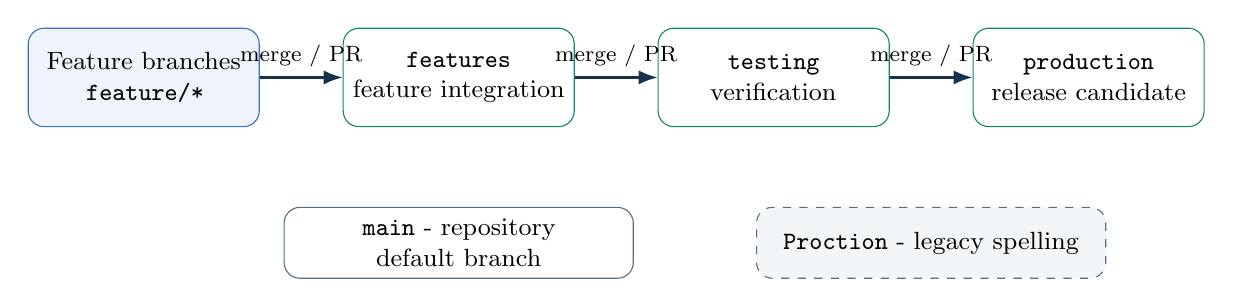
\begin{tikzpicture}[
  branch/.style={draw=JerryBlue,fill=JerryLight,rounded corners=2mm,
    text width=2.7cm,minimum height=1.25cm,align=center,font=\small},
  stage/.style={draw=JerryTeal,fill=white,rounded corners=2mm,
    text width=2.7cm,minimum height=1.25cm,align=center,font=\small},
  flow/.style={-{Latex[length=2.4mm]},thick,draw=JerryNavy}
]
\node[branch] (topic) at (-6,0) {Feature branches\\\code{feature/*}};
\node[stage] (features) at (-2,0) {\code{features}\\feature integration};
\node[stage] (testing) at (2,0) {\code{testing}\\verification};
\node[stage] (production) at (6,0) {\code{production}\\release candidate};
\draw[flow] (topic.east) -- node[above,font=\footnotesize]{merge / PR} (features.west);
\draw[flow] (features.east) -- node[above,font=\footnotesize]{merge / PR} (testing.west);
\draw[flow] (testing.east) -- node[above,font=\footnotesize]{merge / PR} (production.west);
\node[draw=JerryGray,fill=white,rounded corners=2mm,text width=4.2cm,minimum height=0.9cm,align=center,font=\small] (main) at (-2,-2.1) {\code{main} - repository default branch};
\node[draw=JerryGray,dashed,fill=JerryCode,rounded corners=2mm,text width=4.2cm,minimum height=0.9cm,align=center,font=\small] (legacy) at (4,-2.1) {\code{Proction} - legacy spelling};
\end{tikzpicture}%
}
\caption{Intended promotion path for Jerry work. A feature branch is integrated, tested, then promoted to production.}
\label{fig:branches}
\end{figure}

\chapter{Installation and operation}

\section{Prerequisites}
\begin{itemize}
  \item Python 3.11 or later.
  \item PowerShell or another shell capable of running Python and Uvicorn.
  \item Project dependencies from \code{requirements.txt}.
  \item Optional service credentials only when enabling hosted LLM, hosted embeddings, Pinecone, or LangSmith.
\end{itemize}

\section{Install dependencies and configure}
Run commands from the repository root. A virtual environment is recommended.
\begin{lstlisting}[language=bash]
python -m venv .venv
.\.venv\Scripts\Activate.ps1
python -m pip install -r requirements.txt
Copy-Item .env.example .env
\end{lstlisting}
On systems where the activation script is unavailable, activate the environment using the shell-specific command or invoke its Python executable directly. Keep the local \code{.env} file private and do not commit credentials.

\section{Build the local sample index}
In default local mode, no external API key is needed. Run the ingestion script before asking document questions:
\begin{lstlisting}[language=bash]
python scripts/ingest_sample_data.py
\end{lstlisting}
The script loads Markdown metadata, creates overlapping chunks, embeds each chunk with the configured provider, and writes \code{data/local_index.jsonl}. The default chunk size is 900 characters with 120-character overlap. The bundled sample corpus currently has five fictional documents.

\section{Start the API and interface}
Run the API and Streamlit interface in separate terminals, both rooted at the repository directory.
\begin{lstlisting}[language=bash]
uvicorn api.main:app --reload --host 127.0.0.1 --port 8010
\end{lstlisting}
\begin{lstlisting}[language=bash]
streamlit run ui/streamlit_app.py --server.port 8501
\end{lstlisting}
Open \url{http://127.0.0.1:8501/}. The API root is \url{http://127.0.0.1:8010/}, health check is \url{http://127.0.0.1:8010/health}, and interactive OpenAPI documentation is \url{http://127.0.0.1:8010/docs}.

\section{Run the development stack with Docker Compose}
Docker Compose is an alternative local development workflow. Docker Desktop with Linux containers and the Compose plugin is required. The optional local \code{.env} file is read at runtime; it is excluded from the Docker build context and should not be committed. If no \code{.env} exists, the application defaults to local providers and demo tokens.

From the repository root in PowerShell, build the images and start the API and UI in the background:
\begin{lstlisting}[language=bash]
if (-not (Test-Path .env)) { Copy-Item .env.example .env }
docker compose up --build -d
\end{lstlisting}
Create or refresh the sample index:
\begin{lstlisting}[language=bash]
docker compose run --rm ingest
\end{lstlisting}
The ingestion service explicitly uses local embeddings and a local index; it does not require a Pinecone key. Open \url{http://localhost:8501/}; the API health endpoint and documentation are at \url{http://localhost:8010/health} and \url{http://localhost:8010/docs}. Stop and remove the development containers with:
\begin{lstlisting}[language=bash]
docker compose down
\end{lstlisting}
The source bind mount supports development reloads. The defaults use host ports 8010 and 8501; when either host port is occupied, set \code{JERRY_API_PORT} or \code{JERRY_UI_PORT} before invoking Compose. Inside the Compose network, the UI must use \code{http://api:8010} as the backend URL.

\section{Use the chat interface}
\begin{enumerate}
  \item Select a demo account in the sidebar. Its demo token is filled automatically and shown masked.
  \item Ask about a document in the sample corpus, for example: ``What are the policies?'' or ``What caused the settlement delay?''
  \item Review the response. Open \textbf{Sources} to inspect the cited source documents.
  \item Expand \textbf{Agent activity and observability} to inspect graph events.
  \item Ask a short follow-up in the same session, or choose \textbf{Clear conversation memory} to start over.
\end{enumerate}

Figure~\ref{fig:ui-question} shows the application header and question field. The screenshot is a genuine project capture, not a rendered mockup.
\begin{figure}[H]
\centering
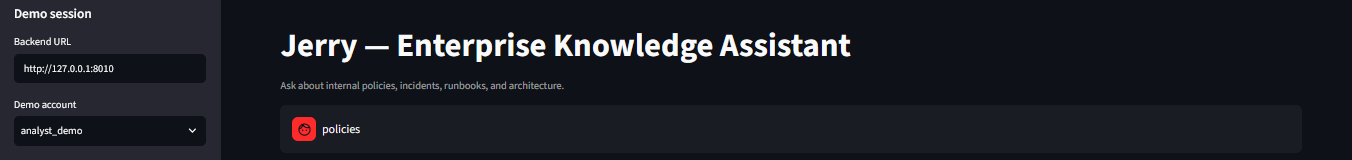
\includegraphics[width=0.98\textwidth]{appsnapshots/01-jerry-chat-controls.png}
\caption{Jerry chat title and a submitted sample question.}
\label{fig:ui-question}
\end{figure}

The sidebar selects a demo account, shows the API URL, and keeps the demo token masked (Figure~\ref{fig:ui-sidebar}).
\begin{figure}[H]
\centering
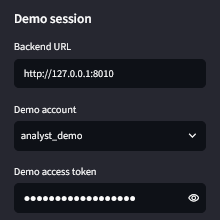
\includegraphics[width=0.35\textwidth]{appsnapshots/02-demo-session-sidebar.png}
\caption{Demo session controls. The displayed identity is a demo account, not a production user.}
\label{fig:ui-sidebar}
\end{figure}

\section{Refresh or select an index backend}
Local ingestion is the default. Pinecone can be selected with \code{--backend pinecone} for ingestion and \code{VECTOR_BACKEND=pinecone} for retrieval. Configure Pinecone API key, index, namespace, and a vector dimension matching the selected embedding provider. The remote index must exist and contain the ingested chunks before retrieval.

\chapter{Configuration}

Settings are read from the process environment and, when present, a local \code{.env} file. The example template should retain local providers and tracing disabled until an operator explicitly configures an external service.

\begin{longtable}{@{}>{\scriptsize\raggedright\arraybackslash}p{49mm}>{\scriptsize\raggedright\arraybackslash}p{36mm}L{55mm}@{}}
\toprule
\textbf{Variable} & \textbf{Local default} & \textbf{Purpose / notes} \\
\midrule
\endfirsthead
\toprule
\textbf{Variable} & \textbf{Local default} & \textbf{Purpose / notes} \\
\midrule
\endhead
\code{APP_NAME} & \code{Jerry} & Application label. \\
\code{APP_ENV} & \code{development} & Environment label for logs. \\
\code{API_HOST} & \code{127.0.0.1} & API bind address. \\
\code{API_PORT} & \code{8010} & API port. \\
\code{API_BASE_URL} & \code{http://127.0.0.1:8010} & Backend URL used by the Streamlit client. \\
\code{LOG_LEVEL} & \code{INFO} & Python logging threshold. \\
\code{EMBEDDING_PROVIDER} & \code{local} & Local feature-hash or optional hosted semantic embedding adapter. \\
\code{OPENAI_API_KEY} & empty & Secret for optional OpenAI chat or embedding APIs. Do not commit. \\
\code{OPENAI_EMBEDDING_MODEL} & \code{text-embedding-3-small} & Embedding model used when the OpenAI adapter is selected. \\
\code{LLM_PROVIDER} & \code{local} & Local extractive response or optional OpenAI chat generation. \\
\code{OPENAI_CHAT_MODEL} & \code{gpt-4o-mini} & Model used by the optional OpenAI chat adapter. \\
\code{VECTOR_BACKEND} & \code{local} & Local JSONL index or Pinecone. \\
\code{PINECONE_API_KEY} & empty & Secret for optional Pinecone access. \\
\code{PINECONE_INDEX} & \code{jerry-demo} & Pinecone index name when selected. \\
\code{PINECONE_NAMESPACE} & \code{jerry-demo} & Pinecone namespace when selected. \\
\code{VIEWER_DEMO_TOKEN} & demo fallback & Viewer demo credential. Replace before any non-local use. \\
\code{ANALYST_DEMO_TOKEN} & demo fallback & Analyst demo credential. Replace before any non-local use. \\
\code{ADMIN_DEMO_TOKEN} & demo fallback & Administrator demo credential. Replace before any non-local use. \\
\code{RATE_LIMIT_CAPACITY} & \code{20} & Token bucket burst capacity per demo user. \\
\code{RATE_LIMIT_REFILL_PER_MINUTE} & \code{10} & Token refill rate per minute per demo user. \\
\code{RETRIEVAL_TIMEOUT_SECONDS} & \code{15} & Configured retrieval timeout. \\
\code{LLM_TIMEOUT_SECONDS} & \code{30} & Configured LLM timeout. \\
\code{TOOL_TIMEOUT_SECONDS} & \code{3} & Timeout for local MCP-style tool calls. \\
\code{LANGSMITH_TRACING} & \code{false} & Tracing is opt-in and also requires an API key. \\
\code{LANGSMITH_API_KEY} & empty & LangSmith secret. Never add a real key to the repository. \\
\code{LANGSMITH_PROJECT} & \code{jerry-assistant} & Project name for optional traces. \\
\code{LANGSMITH_ENDPOINT} & hosted LangSmith API & Optional regional or self-hosted endpoint override. \\
\bottomrule
\end{longtable}

\chapter{Document ingestion and data model}

\section{Source records}
\code{models/documents.py} defines validated \code{DocumentRecord} and \code{DocumentChunk} models. A document includes a stable document ID, title, text, department, document type, access level, and optional creation date. The current access-level values are \code{public}, \code{internal}, and \code{confidential}. Sample metadata is loaded from Markdown header fields.

\section{Chunking and indexing}
Text is whitespace-normalized, split into bounded chunks, and given a configurable overlap. Chunk IDs combine the source document ID and a chunk number. Each index record stores the chunk ID, embedding vector, source text, and retrieval metadata. The local index is a JSONL file intended to be inspectable. Pinecone ingestion uses the same chunk metadata and a configured namespace.

The sample corpus comprises the following fictional reference documents:
\begin{longtable}{@{}L{28mm}L{41mm}L{78mm}@{}}
\toprule
\textbf{Document ID} & \textbf{Type / department} & \textbf{Subject} \\
\midrule
\endfirsthead
\toprule
\textbf{Document ID} & \textbf{Type / department} & \textbf{Subject} \\
\midrule
\endhead
\code{POL-SEC-003} & Security policy / Security & Internal information handling and access responsibilities. \\
\code{INC-2025-014} & Incident / Payments & Delayed settlement after gateway timeouts and queue saturation. \\
\code{INC-2025-022} & Incident / Payments & Duplicate pending authorizations after retries without stable idempotency keys. \\
\code{ARC-PAY-002} & Architecture / Engineering & Payment API, queue, worker, gateway, and idempotency design. \\
\code{RUN-PAY-001} & Runbook / Payments & Operational checks for elevated payment latency and outages. \\
\bottomrule
\end{longtable}

\chapter{Search and retrieval}

\section{Search modes}
Sparse search uses BM25 over the local sample corpus and normalizes simple plurals such as ``policies'' to ``policy''. Dense search reads local vectors or queries Pinecone. When semantic embeddings are configured, the dense and sparse rankings are combined with weighted reciprocal rank fusion (RRF). Raw BM25 and dense similarity scores have different scales; RRF combines ranks rather than adding the raw scores.

With \code{EMBEDDING_PROVIDER=local}, feature-hash vectors are not treated as semantic rankings. The local path therefore uses BM25 alone to avoid arbitrary hash collisions. To use semantic dense retrieval, configure a semantic embedding provider, ingest again, and ensure the Pinecone index dimension matches if Pinecone is enabled.

\section{Metadata filters and citations}
Retrieval filters can constrain department, document type, access level, and inclusive creation-date bounds. Search results carry the source document ID, title, chunk ID, metadata, rank, and component scores. Citation validation only accepts source document IDs among the retrieved evidence.

\chapter{Assistant workflow and analysis}

\section{Grounded chat graph}
The graph validates the request, resolves intent, routes to knowledge retrieval or a selected tool path, assesses whether evidence supports an answer, optionally performs one bounded wider retrieval retry, creates a response, and validates citations. It does not loop indefinitely. In local generation mode, the response is extractive and based on retrieved passages. Optional OpenAI generation is also constrained to retrieved evidence; prompt instructions label retrieved content as untrusted data.

If evidence remains insufficient, Jerry returns a safe no-evidence response rather than inventing policy or operational facts. This is expected when a question is outside the indexed corpus or the index is empty.

\section{Recursive-analysis path}
Analysis-shaped requests are routed through a bounded RLM-style path. It plans a focused incident search, restricts retrieval to incident documents, applies department and date filters when specified, splits passages into batches of at most three, and processes no more than four batches (12 passages). Python helper logic aggregates deterministic cause-pattern signals and source citations.

This is a controlled analysis demonstration, not an autonomous recursively calling language model. Cause labels are keyword and phrase pattern indicators. The returned answer and activity events should be interpreted with that limitation.

\chapter{Session memory, roles, and tools}

\section{Session memory}
The in-process, thread-safe memory store retains at most the latest three user/assistant exchanges for a session and is bounded to 1,000 sessions. Short follow-ups can include the latest prior user question to resolve references. Prior assistant text is context, not factual evidence. Session identity is bound to the server-resolved user and role; a conflicting identity is rejected. Memory resets on API process restart and is not shared across multiple workers.

\section{Role-based access control}
The API validates the \code{X-Demo-Token} header, maps it to a server-side demo identity, and derives the role. The request body does not choose its role. Permission checks are placed at tool execution boundaries; the graph also blocks Viewer analysis before entering the RLM path.

\begin{table}[H]
\centering
\begin{tabularx}{\textwidth}{@{}L{35mm}YYYY@{}}
\toprule
\textbf{Role} & \textbf{Chat / search} & \textbf{Python analysis} & \textbf{MCP-style tools} & \textbf{Admin tools} \\
\midrule
Viewer & Yes & No & No & No \\
Analyst & Yes & Yes & Yes & No \\
Administrator & Yes & Yes & Yes & Yes \\
\bottomrule
\end{tabularx}
\caption{Demo role capability matrix.}
\end{table}

The account selector is a convenience for the local demo, not a production login page or identity provider. Fallback tokens in the example configuration are public demo values; replace them and use an approved authentication system before exposing the service.

\section{Tools}
Knowledge search returns source-linked results. Python analysis accepts one to 12 validated passages and extracts bounded cause signals. Employee and service lookups return fictional local records through an MCP-client-style wrapper. They are not connected to a separate MCP server. The index-status endpoint is administrator-only.

\chapter{API reference}

Except for root and health routes, API access uses \code{X-Demo-Token}. Chat bodies have a query of 1 to 4,000 characters and an optional session ID of 1 to 120 characters. The session ID defaults to \code{demo} if omitted.

{\setlength{\tabcolsep}{2pt}
\begin{longtable}{@{}L{16mm}>{\scriptsize\raggedright\arraybackslash}p{60mm}L{28mm}L{45mm}@{}}
\toprule
\textbf{Method} & \textbf{Path} & \textbf{Access} & \textbf{Purpose} \\
\midrule
\endfirsthead
\toprule
\textbf{Method} & \textbf{Path} & \textbf{Access} & \textbf{Purpose} \\
\midrule
\endhead
GET & \code{/} & Public & Service status and links to health/docs. \\
GET & \code{/health} & Public & Health check. \\
GET & \code{/docs} & Public & Interactive OpenAPI documentation. \\
POST & \code{/api/chat} & Demo token & Non-streaming answer, citations, activity, memory count, and trace metadata. \\
POST & \code{/api/chat/stream} & Demo token & Server-sent events for node activity followed by the final response. \\
DELETE & \code{/api/chat/memory?session_id=...} & Demo token & Clear the current user's session memory. \\
POST & \code{/api/tools/search} & Demo token + search permission & Search with bounded top-k and optional department/type filters. \\
POST & \code{/api/tools/analysis} & Analyst or Administrator & Structured analysis over validated passages. \\
GET & \code{/api/tools/employees} & Analyst or Administrator & Local fictional employee lookup. \\
GET & \code{/api/tools/services} & Analyst or Administrator & Local fictional service lookup. \\
GET & \code{/api/tools/admin/index-status} & Administrator & Local index existence/status. \\
\bottomrule
\end{longtable}
}

\section{Chat request example}
\begin{lstlisting}
{
  "query": "What are the policies?",
  "session_id": "demo-session"
}
\end{lstlisting}
Supply the selected demo token in the HTTP header, not in the JSON body. A successful chat response includes \code{answer}, \code{citations}, \code{activity}, \code{memory_turns}, \code{trace_id}, and tracing status. The exact response fields are defined in \code{models/api.py}.

\chapter{Security and guardrails}

\section{Trust boundaries}
\begin{itemize}
  \item Request schemas bound query and tool-argument sizes. Graph validation rejects malformed control characters and recognized instruction override, secret extraction, permission bypass, and arbitrary command patterns.
  \item Retrieved passages are checked for source identifiers, size, and unsafe patterns before generation or analysis. Retrieved documents are treated as data, not executable instructions.
  \item Tool arguments are schema-validated, and role permissions are checked immediately before execution.
  \item Responses are length-bounded, token-like secrets are redacted, and citations are checked against retrieved document IDs. Invalid citations are removed; a cited extractive fallback is available if a grounded response omitted citations.
\end{itemize}

\section{Limitations and safe use}
The injection detector uses phrase patterns. Obfuscation and novel attack wording may evade it; benign passages may also match. These controls are defense in depth and are not a security guarantee. Demo users, local tokens, process memory, and local logs are not a production security architecture. Do not use real customer or confidential information in this assignment demo. LangSmith can retain model inputs, outputs, and retrieved evidence when tracing is enabled; send synthetic data unless appropriate organizational controls approve otherwise.

\chapter{Reliability and observability}

\section{Rate limits}
Authenticated chat and tool routes use a per-user token bucket. Defaults allow a burst of 20 requests and refill 10 tokens per minute. A rejected request returns HTTP 429 and a \code{Retry-After} header. Root and health endpoints remain available. The limiter is process-local; multi-worker or multi-host deployments need a shared state store such as Redis.

\section{Timeouts and error mapping}
Retrieval, LLM, and tool timeouts are configurable. A tool timeout returns a safe timeout response. OpenAI failures can fall back to cited extractive output. Unexpected errors are logged with a trace ID while the client receives a generic message.

\begin{table}[H]
\centering
\begin{tabularx}{\textwidth}{@{}L{23mm}Y@{}}
\toprule
\textbf{HTTP status} & \textbf{Typical meaning} \\
\midrule
401 & Missing or invalid demo token. \\
403 & Authenticated demo role lacks permission for the requested tool. \\
409 & A memory session is being reused with a conflicting user or role identity. \\
422 & Request or tool parameters do not satisfy the schema or size constraints. \\
429 & Per-user request limit reached; inspect \code{Retry-After}. \\
500 & Unexpected server failure; provide the trace ID to the maintainer. \\
503 & Assistant or downstream service is unavailable. \\
504 & A bounded MCP-style tool call exceeded its timeout. \\
\bottomrule
\end{tabularx}
\caption{Common error responses. Exact details can depend on the route and failure.}
\end{table}

\section{LangSmith and streamed activity}
Tracing is enabled only when \code{LANGSMITH_TRACING=true} and a non-empty \code{LANGSMITH_API_KEY} are configured. Graph runs carry a name, tags, role/user/session metadata, and trace ID. Retrieval, Python analysis, and local MCP-style wrappers can appear as child runs. The Streamlit client consumes \code{POST /api/chat/stream}, which emits activity events as server-sent events and then a final response. Non-streaming clients can use \code{POST /api/chat}.

The event panel can be reviewed in Figure~\ref{fig:activity}. It represents an earlier captured run; the displayed no-evidence outcome is not the expected answer for every query.
\begin{figure}[H]
\centering
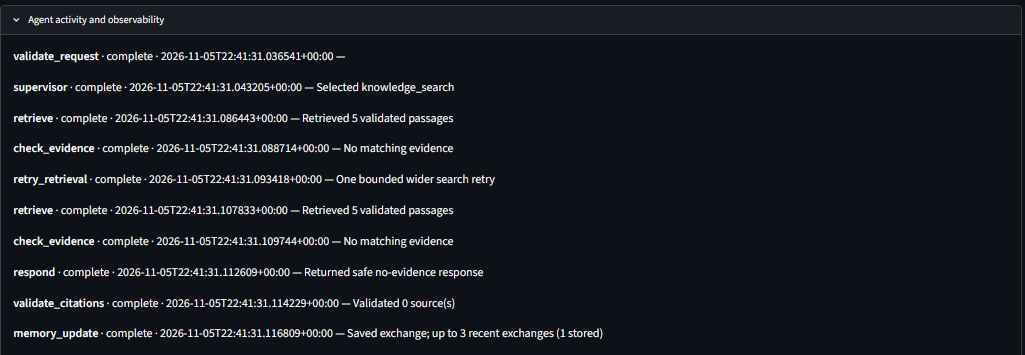
\includegraphics[width=\textwidth]{appsnapshots/03-agent-activity-panel.png}
\caption{Expanded activity panel showing graph steps.}
\label{fig:activity}
\end{figure}

\chapter{Testing and verification}

\section{Recorded local result}
The test record dated November 6, 2026 reports 10 feature areas plus the Streamlit UI smoke check: 11 checks passed and zero failed. The local API root, health endpoint, OpenAPI docs, and Streamlit page each returned HTTP 200. The local sample corpus contained five documents and five indexed chunks.

{\setlength{\tabcolsep}{3pt}
\begin{longtable}{@{}>{\bfseries}L{6mm}L{32mm}L{92mm}L{12mm}@{}}
\toprule
\textbf{No.} & \textbf{Feature} & \textbf{Recorded check} & \textbf{Result} \\
\midrule
\endfirsthead
\toprule
\textbf{No.} & \textbf{Feature} & \textbf{Recorded check} & \textbf{Result} \\
\midrule
\endhead
1 & Project foundation & Root, health, and API docs respond; protected tools reject a missing token with 401. & PASS \\
2 & Ingestion and data model & Five Markdown documents loaded and five metadata-bearing chunks generated. & PASS \\
3 & Hybrid retrieval & Policy query returns \code{POL-SEC-003}; department filtering returns payment documents. & PASS \\
4 & LangGraph flow & Grounded chat returns a citation and workflow activity events. & PASS \\
5 & Recursive analysis & Analyst incident summary returns RLM activity/citations; batches are at most 3 and capped at 4. & PASS \\
6 & Session memory & Follow-up retains session context and clear-memory succeeds. & PASS \\
7 & RBAC and tools & Viewer denied analysis/admin; Analyst analysis and employee tool allowed; Administrator index status allowed. & PASS \\
8 & Security & Injection rejection, retrieved-content screening, secret redaction, and invalid-citation removal exercised. & PASS \\
9 & Resilience & Oversized query returns 422; rate-limited request returns 429 with \code{Retry-After}. & PASS \\
10 & Observability & Streaming activity and final events plus trace ID verified. Remote export was disabled. & PASS* \\
UI & Streamlit interface & AppTest renders title and chat input without app exception. & PASS \\
\bottomrule
\end{longtable}
}
\textit{* Local stream and trace-ID behavior was exercised; no LangSmith trace was sent.}

\section{Coverage not established}
The recorded run did not contact Pinecone, hosted semantic embeddings, an external MCP server, or the LangSmith service. It does not establish retrieval performance on a larger corpus, multi-worker behavior, deployment security, or production availability. AppTest emitted its standard bare-mode \code{ScriptRunContext} warning but no application exception.

\section{Docker development verification}
On November 7, 2026, the Docker Compose development path was checked on Windows with Docker Desktop 29.9.2 and Compose 5.6.1. The images built successfully, both application services ran, and the API health check reported healthy.

\begin{tabularx}{\textwidth}{@{}L{58mm}Y@{}}
\toprule
\textbf{Check} & \textbf{Observed result} \\
\midrule
Docker Engine / Compose versions & 29.9.2 / 5.6.1 \\
Compose image build & PASS; API and UI images built \\
API container health & Healthy \\
\code{GET /health} & HTTP 200 \\
\code{GET /docs} & HTTP 200 \\
Streamlit at host port 8501 & HTTP 200 \\
UI container to \code{http://api:8010/health} & HTTP 200; Compose DNS path works \\
Local ingestion service & PASS; 5 sample documents and 5 chunks indexed \\
Authenticated chat request & HTTP 200; 1 citation and a trace ID returned \\
\bottomrule
\end{tabularx}

These results establish a local development smoke test only. The trace ID does not by itself establish remote LangSmith delivery, and this run does not assess production security or external provider integrations. The detailed record is \code{docs/testing/docker-testing.md}.

\section{Repeat the manual checks}
\begin{enumerate}
  \item Run \code{python scripts/ingest_sample_data.py} from the repository root.
  \item Start Uvicorn on port 8010 and Streamlit on port 8501 in separate terminals.
  \item Open \url{http://127.0.0.1:8501/}, select a demo role, and ask ``What are the policies?''
  \item Confirm the source citation, then use Analyst for analysis and local tool checks and Administrator for index status.
  \item Use \url{http://127.0.0.1:8010/docs} for request schemas and route exploration.
\end{enumerate}
The detailed record and known limitations are maintained in \code{docs/testing/testing.md} and \code{docs/testing/role-based-testing.md}.

\chapter{Troubleshooting}

\begin{longtable}{@{}L{40mm}L{106mm}@{}}
\toprule
\textbf{Symptom} & \textbf{Action} \\
\midrule
\endfirsthead
\toprule
\textbf{Symptom} & \textbf{Action} \\
\midrule
\endhead
Streamlit cannot connect & Keep both processes running. Check \url{http://127.0.0.1:8010/health} and confirm the sidebar Backend URL is correct. \\
No supporting documents & Run the ingestion script from the repository root. Verify the local index exists and try a question matching one of the five sample documents. \\
\code{ModuleNotFoundError} for a project package & Launch Streamlit from the repository root with \code{streamlit run ui/streamlit_app.py}. \\
HTTP 401 & Verify the selected demo token is present and matches the configured server-side token. \\
HTTP 403 & Use a role permitted to perform the operation. This is expected for Viewer requests to analysis or admin tools. \\
HTTP 409 & Start a fresh session if the user identity or role has changed. \\
HTTP 422 & Check required fields, text lengths, and the schema in \url{http://127.0.0.1:8010/docs}. \\
HTTP 429 & Wait for the per-user token bucket to refill; inspect \code{Retry-After}. \\
Docker port already in use & Change \code{JERRY_API_PORT} or \code{JERRY_UI_PORT}, then restart the Compose stack. \\
UI cannot reach API in Docker & Set the UI backend URL to \code{http://api:8010}; \code{localhost} inside a container is that same container. \\
Tracing disabled & Configure the explicit enable flag and key in a private \code{.env} file. Do not commit the key. \\
\bottomrule
\end{longtable}

\chapter{Deployment considerations}

Before using any hosted environment, replace fallback demo tokens, introduce a production identity provider, protect secrets with a managed secret store, and configure TLS and network access controls. Move session state and rate-limit buckets to shared durable infrastructure when using multiple workers. Establish document-level authorization and audit policy for real information. Validate prompt-injection controls with the organization's threat model. Decide what telemetry can be sent to LangSmith and configure retention/region settings accordingly. Configure and test each external provider independently. The current implementation and test evidence are for a local assignment/demo, not a production readiness certification.

\chapter{Glossary and source documents}

\section{Glossary}
\begin{description}[style=nextline,leftmargin=29mm,labelwidth=26mm]
  \item[BM25] A keyword-ranking function used by the sparse local search implementation.
  \item[Chunk] A bounded text section derived from a source document and retained with source metadata.
  \item[LangGraph] The graph orchestration library used to construct and stream assistant workflow nodes.
  \item[LangSmith] Optional tracing and observability service for graph and tool executions.
  \item[MCP] Model Context Protocol. Jerry's current employee/service integrations are local MCP-style wrappers, not a remote MCP server.
  \item[RLM-style] A bounded recursive-analysis-inspired process in this project; it uses focused retrieval, capped passage batches, and deterministic Python analysis.
  \item[RBAC] Role-based access control: tool permissions are derived from the server-resolved role.
  \item[RRF] Reciprocal rank fusion, a method for combining ranked candidate lists.
  \item[SSE] Server-sent events, used by the streaming chat endpoint to report node updates and the final response.
\end{description}

\section{Repository documentation references}
This manual consolidates information from the following repository sources. They remain the detailed, component-level notes:
\begin{itemize}
  \item \code{docs/architecture.md} and \code{docs/development-flow.md}
  \item \code{docs/ingestion.md} and \code{docs/retrieval.md}
  \item \code{docs/assistant-flow.md} and \code{docs/recursive-analysis.md}
  \item \code{docs/session-memory.md} and \code{docs/testing/role-based-testing.md}
  \item \code{docs/security-guardrails.md} and \code{docs/resilience.md}
  \item \code{docs/observability.md} and \code{docs/testing/testing.md}
  \item \code{Dockerfile}, \code{docker-compose.yml}, and \code{docs/testing/docker-testing.md}
\end{itemize}

\appendix
\chapter{Compile this LaTeX source}
Install a LaTeX distribution that includes pdfLaTeX and the packages listed in the preamble (including TikZ). From the repository root, compile twice so the table of contents and cross-references settle:
\begin{lstlisting}[language=bash]
pdflatex -interaction=nonstopmode docs/jerry-software-documentation.tex
pdflatex -interaction=nonstopmode docs/jerry-software-documentation.tex
\end{lstlisting}
The resulting PDF is written next to the source. Figure paths are relative to the repository root. The PDF contains static screenshots; the animated walkthrough remains in the README as a GIF.

\end{document}
